\section{Methodology \& Implementation}\label{sec:meths}

\subsection{Harmonization Methods}

IAM emission results are provided along temporal (normally half decade or
decade), spatial (i.e., model regions), gas species, and sectoral
dimensions. Each individual temporal trajectory, i.e., unique combinations of
regions ($r$), species ($g$), and sectors ($s$), must be harmonized to the
initial starting point. Given a model trajectory, $m_{r, g, s}(t)$, historical
values, $h_{r, g, s}(t)$, and initial starting point $t_i$, a harmonized
trajectory needs to be calculated. The ``goodness of fit'' of a trajectory depends on
% * <maarten.vandenberg@pbl.nl> 2017-07-03T21:16:50.244Z:
% 
% Assessing the "goodness of fit" is not  straightforward, there may be competing factors. Perhaps we should refer back to this in the discussion. 
% 
% ^.
a number of factors, most notably the faithful representation of the original,
unharmonized, trajectory. However, other important factors must be considered,
such as the representation of negative trajectories (i.e., if a trajectory
becomes negative, both the timing and total magnitude should be as close as
possible) which are of critical importance for cumulative CO2 calculations.
% * <ssmith@pnnl.gov> 2017-07-01T03:25:04.357Z:
% 
% Suggest moving this later where negative emissions are discussed. Its a bit of a tangent here.
% 
% ^ <ssmith@pnnl.gov> 2017-07-01T03:25:44.627Z.

In previous studies \cite{meinshausen_rcp_2011,rogelj_discrepancies_2011}, two
\textit{families} of methods have been used: those that operate on the ratio of
base year values (i.e., $\frac{h(t_i)}{m(t_i)}$) and those that operate on the
offset of base year values (i.e., $h(t_i) - m(t_i)$). The \code{aneris} code
base provides a number of implementations on the classic methods, including
% * <maarten.vandenberg@pbl.nl> 2017-07-03T21:27:39.375Z:
% 
% > classic methods
% This might be interpreted as that convergence have not been previously applied. Perhaps use " implementations"  instead of "variations" .
% 
% ^.
ratio-convergence methods shown in Equation \ref{eqs:ratio}, offset-convergence
methods shown in Equation \ref{eqs:offset}, and interpolation methods shown in
Equation \ref{eqs:interpolate}; the convergence factor, $\beta$, for associated
methods is shown first in Equation \ref{eqs:factor}. Note that region, species,
and sector indices have been dropped for clarity. Each equation is a function of
time, model trajectory, historical trajectory, harmonization time step, and a
convergence time step ($t_f$), at which point the harmonized trajectory
converges to the unharmonized trajectory. The \code{aneris} code base provides a
number of methods to choose from for each of the harmonization families. A
summary of all available methods is provided in Table \ref{tab:meths}.
% * <maarten.vandenberg@pbl.nl> 2017-07-03T21:34:25.905Z:
% 
% > A
% > summary
% If beta would be defined as \frac{t -t_i}{t_f - t_i}, it might better match intuition of convergence: 0 value at t = t_i and 1 at full convergence (t = t_f), with added benefit the beta parameter can also be used in the interpolation option.
% 
% ^.


\begin{equation}\label{eqs:factor}
  \beta(t, t_i, t_f) =
  \begin{cases}
    1 - \frac{t - t_i}{t_f - t_i},& \text{if } t \leq t_f\\
    0,                        & \text{otherwise}
  \end{cases}
\end{equation}

\begin{equation}\label{eqs:ratio}
  m^{rat}(t, m, h, t_i, t_f) = [\beta(t, t_i, t_f) (\frac{h(t_i)}{m(t_i)} - 1) + 1] m(t)
\end{equation}

\begin{equation}\label{eqs:offset}
  m^{off}(t, m, h, t_i, t_f) = \beta(t, t_i, t_f) (h(t_i) - m(t_i)) + m(t)
\end{equation}
  
\begin{equation}\label{eqs:interpolate}
  m^{int}(t, m, h, t_i, t_f) =
  \begin{cases}
    \beta(t, t_i, t_f) (h(t_i) - m(t_f)) + m(t_f), & \text{if } t \leq t_f\\
    m(t), & \text{otherwise}
  \end{cases}
\end{equation}


\begin{table}[h!]
\centering
\caption{All Harmonization Methods Provided in \code{aneris}}
\label{tab:meths}
\begin{tabular}{|l|l|l|}
\hline
Method Name                             & Harmonization Family & Convergence Year\\
\hline
\code{constant\_ratio}                  & ratio              & $t_f = \infty$\\
\code{reduce\_ratio\_<year>}            & ratio              & $t_f = $\code{<year>}\\
\code{constant\_offset}                 & offset             & $t_f = \infty$\\
\code{reduce\_offset\_<year>}           & offset             & $t_f = $\code{<year>}\\
\code{linear\_interpolate\_<year>}      & interpolation      & $t_f = $\code{<year>}\\
\hline
\end{tabular}
\end{table}

\subsection{Default Method Decision Tree}\label{sec:tree}

While historically expert opinion has guided the choice of harmonization methods
for a given trajectory, a new, \textit{decision tree} approach has been
implemented in this work which provides a systematic and documented
decision-making process for method determination. In order to provide reasonable
\textit{default} methods, the historical trajectory, unharmonized model
trajectory, and relative difference between history and model values in the
harmonization year are analyzed. The decision tree used in this analysis is
shown graphically in Figure \ref{fig:decision_tree}.


\begin{figure}
  \begin{center}
    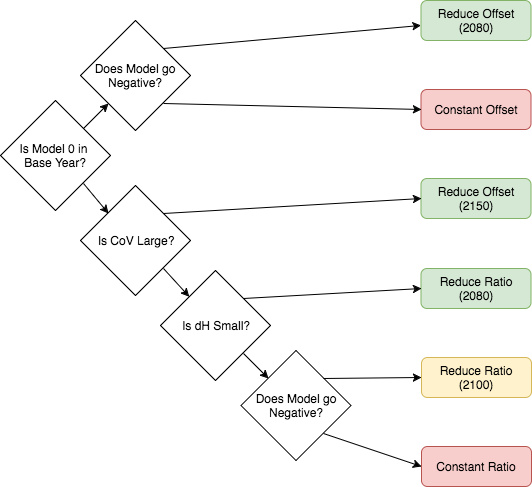
\includegraphics[width=\textwidth]{decision_tree.png}
    \caption[]{
      \label{fig:decision_tree}
      The default method decision tree used in the \code{aneris} software
% * <maarten.vandenberg@pbl.nl> 2017-07-03T21:40:43.868Z:
% 
% > The default method decision tree
% yes and no might be added to the tree for improved clarity. 
% 
% ^.
      library. For all decisions, upper branches represent a ``yes'' response
      and lower branches represent a ``no'' response. $dH$ is defined as
      $\left|\frac{h(t_i) - m(t_i)}{h(t_i)}\right|$, and decision-making
      thresholds are described below. Finally, default choices in \textit{green}
% * <maarten.vandenberg@pbl.nl> 2017-07-03T21:42:35.965Z:
% 
% for CoV and dH
% 
% ^.
      label methods that will likely closely match unharmonized results, choices
      in \textit{yellow} will likely somewhat match unharmonized results, and
      choices in \textit{red} can be expected to have a large relative
      difference between harmonized and unharmonized results.}
  \end{center}
\end{figure}

A number of characteristics impact the decision of which default method to
select based on the effect of the characteristic on the potential harmonized
trajectory. For example, it is possible for models to report zero values in the
harmonization year in situations in which technologies are introduced in future
time periods in regions or for sectors which produce an emissions species that
is absent in the initial modeling period. In such cases, an offset method is
required as a ratio method would mask future emissions and erroneously harmonize
the trajectory. 

In most cases, however, models do report values in the harmonization
year. Figure \ref{fig:cases} displays a number of example trajectories which
highlight the possible issues resulting from harmonizing model results in
different contexts. When model and historical values are relatively close, a
convergence method is chosen in order to be as representative as possible to the
underlying unharmonized model results (Figure \ref{fig:cases}, Panel
\code{a}). If values are not close, the constant ratio method is chosen in order
to provide reasonable trajectories that still incorporate modeled effects
(Figure \ref{fig:cases}, Panel \code{b}). 

Models can additionally report negative emissions in certain contexts which much
be taken into account during harmonization. Such a case is possible for gas
species which can be extracted from the environment and stored, as is the case
for CO2 in future scenarios with climate mitigation. If a model provides a
trajectory that transitions from positive to negative emissions and base year
results are similar, then a convergence method is used in order to guarantee
capture of this transition in a representative fashion (Figure \ref{fig:cases},
Panel \code{c}). If the discrepancy in base year results is large, it is
possible for a negative trajectory to be inappropriately harmonized to a
positive, but decreasing, trajectory. As such, the constant ratio method is
chosen (Figure \ref{fig:cases}, Panel \code{d}).

\begin{figure}
  \begin{center}
    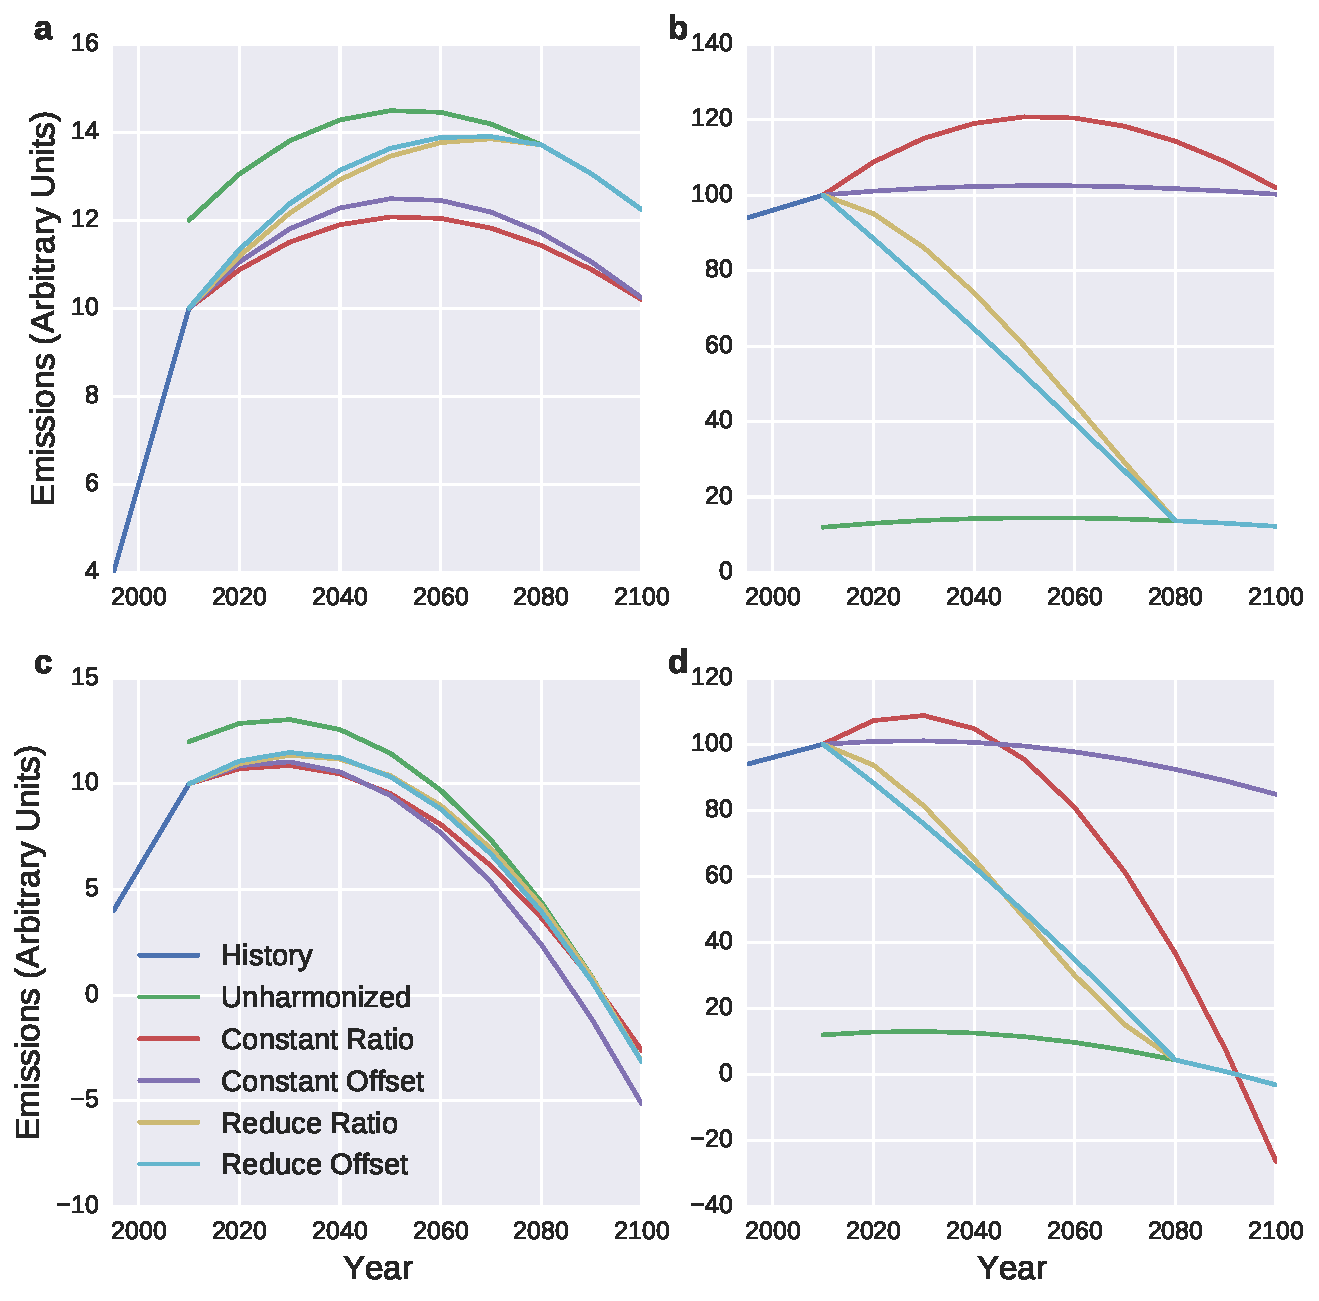
\includegraphics[width=\textwidth]{cases.pdf}
    \caption[]{
      \label{fig:cases}
      The effect of different harmonization routines on model trajectories under
      ``normal'' circumstances (Panel \code{a}), when there is a large
      difference between historical and model values in the harmonization year
      (Panels \code{b} and \code{d}), and when model trajectories result in
      negative emissions by the end of the modeling time horizon (Panels
      \code{c} and \code{d}). In each figure row (Panels \code{a}, \code{b};
      \code{c}, \code{d}), identical model trajectories are used. In each figure
      column, historical values are increased in the base year by an order of
      magnitude (from 10 to 100). In each case, a subset of the potential
      routines provide a better ``goodness of fit'' than others as described in
      the text.  }
  \end{center}
\end{figure}

Temporal variability of the historical trajectory is also an important characteristic
when considering the choice of harmonization method.  Emissions from forest and grassland fires, for example, vary from year to year due to a combination of meteorological conditions and anthropogenic drivers. Land use emissions are modeled by IAMs using average emission factors and do not capture conditions in a specific year.  Ratio methods for such sectors can lead to unrealistic harmonization results.
% * <maarten.vandenberg@pbl.nl> 2017-07-03T21:59:54.238Z:
% 
% > Ratio methods for such sectors can lead to unrealistic harmonization results.
% However, using for instance an offset method may also misrepresent the emission levels. Depending on the trajectory the emission factor can be subject to unintentional changes over the century.
% 
% ^.
modeled with varying fidelity by IAMs, but in general proxies are used for
emissions trajectories. Take for example emissions from grassland burning: for
most models, the use of grass and paturelands is endogenously modeled, and
emissions from the burning of these lands is determined by applying an emissions
factor; in general, the more grassland usage that occurs in a scenario, the
higher the emissions from the burning thereof. Therefore, consistency in
harmonization method is important because the effects are modeled similarly
across regions and species. In order to detect land-use-like emissions,
% * <ssmith@pnnl.gov> 2017-07-01T03:31:52.910Z:
% 
% > modeled with varying fidelity by IAMs, but in general proxies are used for
% > emissions trajectories. Take for example emissions from grassland burning: for
% > most models, the use of grass and paturelands is endogenously modeled, and
% > emissions from the burning of these lands is determined by applying an emissions
% > factor; in general, the more grassland usage that occurs in a scenario, the
% > higher the emissions from the burning thereof. Therefore, consistency in
% > harmonization method is important because the effects are modeled similarly
% > across regions and species. 
% 
% Not sure I follow the logic here. I added some new text that might help. Perhaps the intermediate part could be deleted.
% 
% ^ <ssmith@pnnl.gov> 2017-07-01T03:32:30.453Z.
a measure of the coefficient of variation of the first derivative of the
historical trajectory, $c_v$, is calculated as shown in Equation \ref{eqs:cov},
where $\sigma$ is the standard deviation, and $\mu$ is the mean of the
trajectory.

The value of $c_v$ is then tested against a threshold. To determine this
threshold, an analysis of the recent CEDS and LUC historical data has been
performed. Figure \ref{fig:cov} shows the distribution of LUC $c_v$s and non-LUC
$c_v$s as determined for historical data aggregated to the model regions of 5
different IAMs \TODO{list here or elsewhere?}. A threshold value of 20 has been chosen based on these
observations as it optimally divides the two distributions. Importantly, tails
of the LUC and non-LUC overlap, thus there are both false positives (~10\% of
non-LUC trajectories) and false negatives (~7\% of LUC trajectories). However,
% * <maarten.vandenberg@pbl.nl> 2017-07-03T22:07:21.157Z:
% 
% >  (~10\% of
% > non-LUC trajectories) and false negatives (~7\% of LUC trajectories)
% visually it seems to be that the false negatives are a larger share thatn the false positives?
% 
% ^.
as any regional definition is model dependent and thus any regional aggregation
is possible an automated detection mechanism is necessary.

\begin{equation}\label{eqs:cov}
% * <maarten.vandenberg@pbl.nl> 2017-07-03T22:08:21.230Z:
% 
% > \begin{equation}\label{eqs:cov}
% >     c_v =  \frac{\sigma(h^{\prime}(t))}{\mu(h^{\prime}(t))}
% > \end{equation}
% c_v is called a covariance parameter and a variance of derivatives, what is exactly calculated?
% 
% ^.
    c_v =  \frac{\sigma(h^{\prime}(t))}{\mu(h^{\prime}(t))}
\end{equation}


\begin{figure}
  \begin{center}
    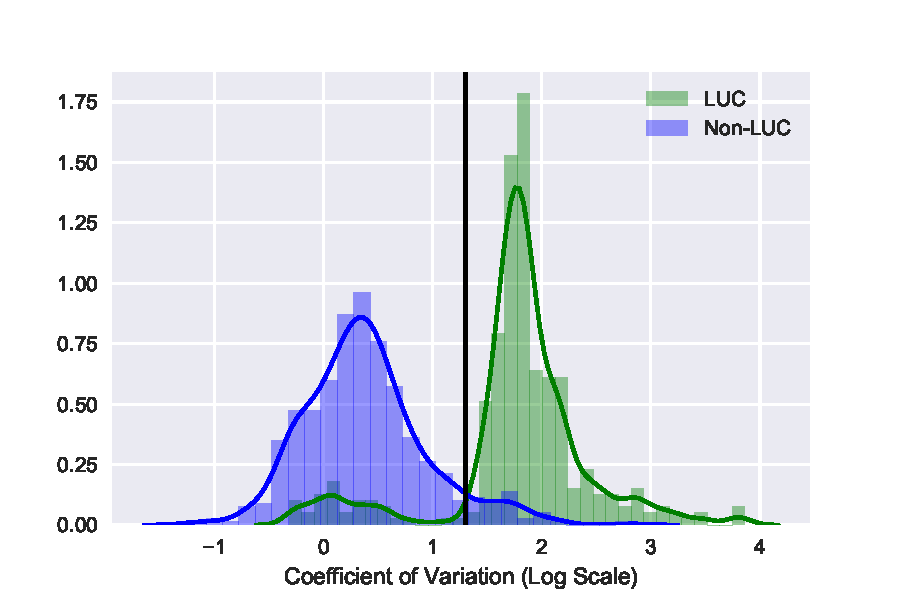
\includegraphics[width=\textwidth]{cov.pdf}
    \caption[]{
      \label{fig:cov}
      The distribution of $c_v$ values for LUC and non-LUC historical
      trajectories is shown. CEDS historical data \cite{hoesly_historical_2017}
      is used for non-LUC data and \cite{van_marle_historic_2017} is used for
      LUC data. All historical data has been aggregated from countries to IAM
      model regional definitions, and all gas species included in the historical
      datasets are included in the analysis. The solid black line indicates the
      threshold value used by default in \code{aneris}.  }
  \end{center}
\end{figure}

Finally, consideration is taken with respect to the relative difference between
the historic and model values in the harmonization time period. In order to
investigate the possible values that these relative differences can take, the
IAM values used in the SSP and (ongoing) CMIP6 inter-comparison
exercises are used. A distribution of these differences for all models in the
study is presented in Figure \ref{fig:dh}. Given the available data, a threshold
value of 50\% was chosen to be used as a default in \code{aneris}.
% * <maarten.vandenberg@pbl.nl> 2017-07-03T22:25:47.452Z:
% 
% > 50\%
% What does this mean? I would expect something of the form low_value < dH < high_value?
% 
% ^.

\begin{figure}
  \begin{center}
    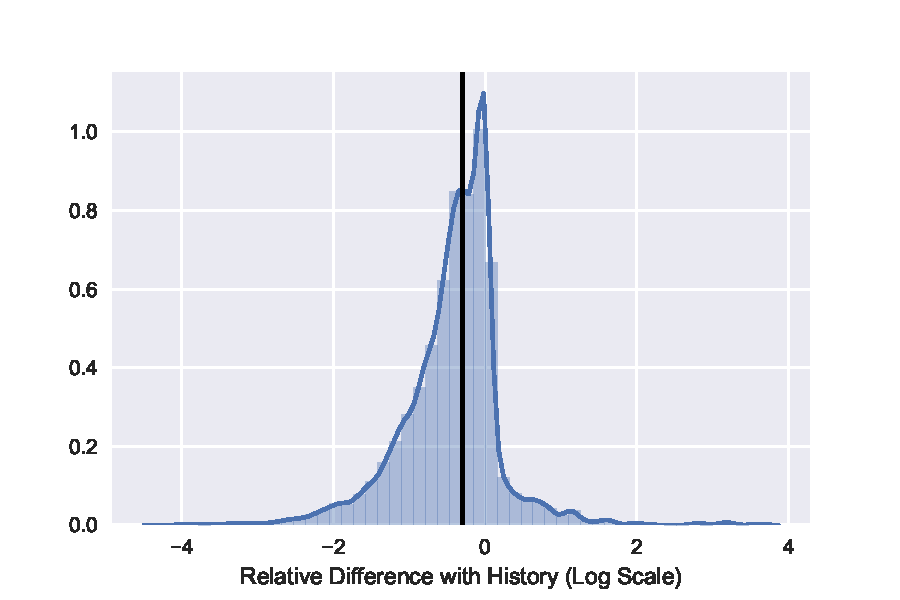
\includegraphics[width=\textwidth]{dh.pdf}
    \caption[]{
      \label{fig:dh}
      The distribution of relative differences between model and historical
      values in the harmonization year is shown. The solid black line indicates
      the 50\% threshold value used by default in \code{aneris}.  
% * <maarten.vandenberg@pbl.nl> 2017-07-03T22:14:59.644Z:
% 
% > The distribution of relative differences between model and historical
% >       values in the harmonization year is shown. The solid black line indicates
% >       the 50\% threshold value used by defaul
% the asymmetry here might be interesting, do the SSP scenarios consistently underestimate emission levels, or is this an effect of history up to 2015, while scenarios start earlier (might not be interesting for this paper).
% 
% ^.
    }
  \end{center}
\end{figure}

\subsection{\code{aneris} Workflow}\label{sec:workflow}

The full \code{aneris} workflow is comprised of a number of components shown
graphically in Figure \ref{fig:workflow}. Unharmonized model data and a
run-control configuration are read in via an Excel spreadsheet. Data is assumed
to be in the \textit{IAM Consortium} format, i.e., using \code{Model},
\code{Scenario}, \code{Region}, \code{Variable}, and \code{Unit} columns in
addition to columns representing each modeled time period. 

Users are able to control the harmonization process via a number of options. The
primary mechanism by which users control the process is by providing
\textit{override} methods for any combination of region and variable (i.e.,
sector and gas species).  In practice, it may be possible that not all default
methods chosen will provide robust harmonized trajectories, especially if there
is a significant difference between historical and model values in the
harmonization year and there is significant upward or downward movement in the
model trajectory. In such cases, override methods can ameliorate the issues
associated with the default method choice. In order to help identify these
cases, harmonization \textit{diagnostics} are provided which analyze the relative
difference between harmonized and unharmonized trajectories at their mid and
end-points. If override methods are provided, they are used instead of the
default methods as determined by the default method decision tree. Furthermore,
users can set the above-mentioned thresholds as well as the LUC method used in
the decision tree (see Figure \ref{fig:decision_tree}). Further detail of input
parameters can be found \href{http://mattgidden.com/aneris/config.html}{online}.

\begin{figure}
  \begin{center}
    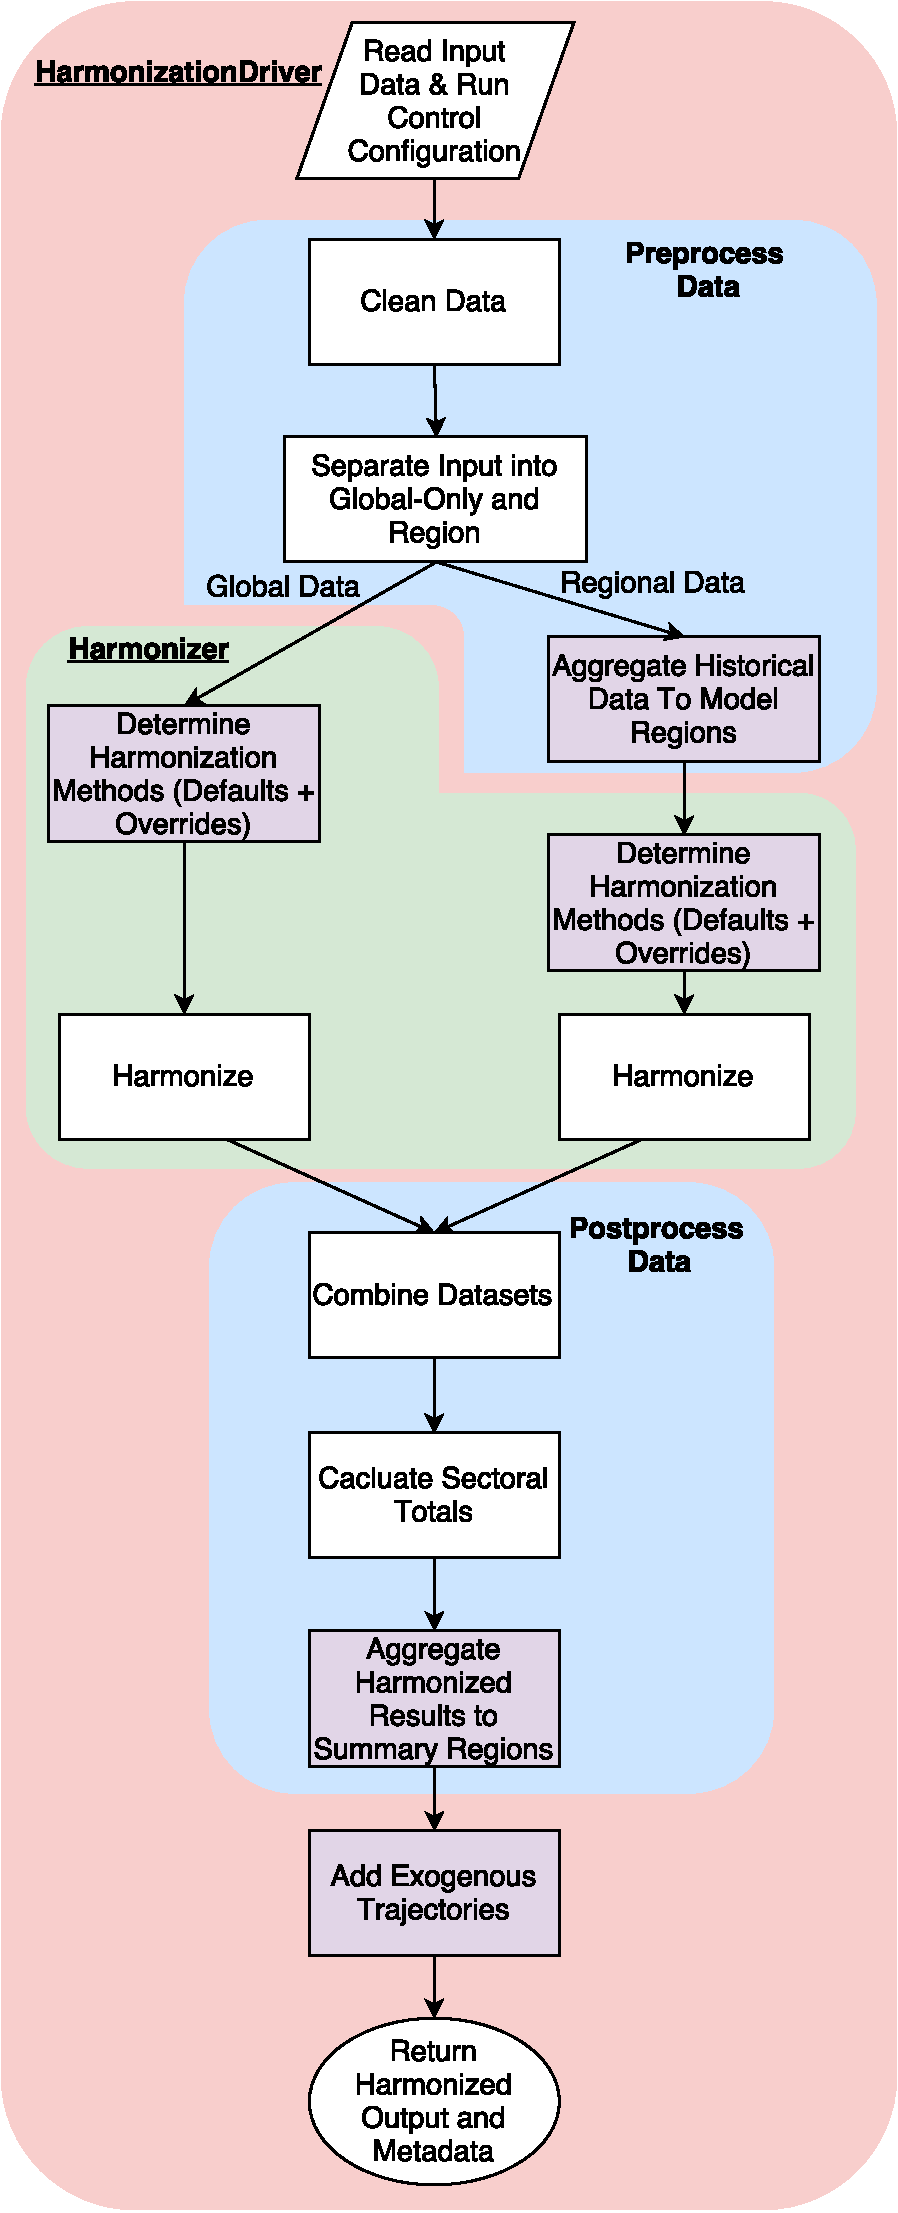
\includegraphics[height=0.85\textheight]{aneris-workflow.pdf}
    \caption[]{
      \label{fig:workflow}
      The full harmonization process as executed by \code{aneris}. Operations
      that can be configured with user-based input configurations are shown in
      purple. The core harmonization process is shown in yellow.  }
  \end{center}
\end{figure}

Input data then undergoes a cleaning operation, which adds (null) model
trajectories that exist in the historical dataset but are not provided by the
model input and detects any issues that would cause the harmonization process to
fail. The methods used to harmonize the data are then determined and the
harmonization process is executed. Upon completion of the harmonization process,
aggregation of common analysis regions is performed. A common regional
aggregation used in the IAM community is the RCP regional definition, as shown
in Figure \ref{fig:regions}. Finally, any exogenous trajectories the user provides
are added. Exogenous trajectories are normally provided for unmodeled gases with
well-accepted scenario trajectories, e.g., chlorofluorocarbons provided by WMO
\cite{wmo2014}. Upon completion, the harmonized trajectories and meta data
regarding the harmonization process are returned. A description of all returned
meta data is provided in Table \ref{tab:metadata}.


\begin{figure}
  \begin{center}
    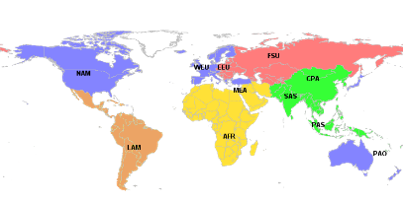
\includegraphics[width=0.85\textwidth]{regions.png}
    \caption[]{
      \label{fig:regions}
      The 5 regions used in the RCPs with their 11-region constituents: Asia
      (Central Asia, South Asia, Pacific Asia), Latin America, the Middle East
      and Africa, the OECD (North America, Western Europe, and Pacific OECD),
      Reforming Economies (Eastern Europe and Former Soviet Union).
    }
  \end{center}
\end{figure}


\begin{table}[]
\centering
\caption{Meta data provided by the \code{aneris} harmonization routine. This meta data is provided for every combination of region, sector, and emissions species.}
\label{tab:metadata}
\begin{tabular}{|p{2cm}|p{8cm}|}
\hline
Column       & Description                                                                  \\
\hline
\hline
method       & The harmonization method used.                                               \\
\hline
default      & The default harmonization method as determined by the default decision tree. \\
\hline
override     & The method provided as an override (if any).                                 \\
\hline
offset       & The offset value between history and model in the harmonization year.        \\
\hline
ratio        & The ratio value between history and model in the harmonization year.         \\
\hline
cov          & The coefficient of variation value of the historical trajectory.                           \\
\hline
unharmonized & The unharmonized value in the harmonization year.                            \\
\hline
history      & This historical value in the harmonization year.                             \\
\hline
harmonized   & The resulting harmonized value in the harmonization year.\\
\hline
\end{tabular}
\end{table}
